%%%%%%%%%%%%%%%%%%%%%%%%%%%%%%%%%%%%%%%%%
% Short Sectioned Assignment LaTeX Template Version 1.0 (5/5/12)
% This template has been downloaded from: http://www.LaTeXTemplates.com
% Original author:  Frits Wenneker (http://www.howtotex.com)
% License: CC BY-NC-SA 3.0 (http://creativecommons.org/licenses/by-nc-sa/3.0/)
%%%%%%%%%%%%%%%%%%%%%%%%%%%%%%%%%%%%%%%%%

%----------------------------------------------------------------------------------------
%	PACKAGES AND OTHER DOCUMENT CONFIGURATIONS
%----------------------------------------------------------------------------------------

\documentclass[paper=a4, fontsize=11pt]{scrartcl} % A4 paper and 11pt font size

% ---- Entrada y salida de texto -----

\usepackage[T1]{fontenc} % Use 8-bit encoding that has 256 glyphs
\usepackage[utf8]{inputenc}
%\usepackage{fourier} % Use the Adobe Utopia font for the document - comment this line to return to the LaTeX default

% ---- Idioma --------

\usepackage[spanish, es-tabla]{babel} % Selecciona el español para palabras introducidas automáticamente, p.ej. "septiembre" en la fecha y especifica que se use la palabra Tabla en vez de Cuadro

% ---- Otros paquetes ----

\usepackage{url} % ,href} %para incluir URLs e hipervínculos dentro del texto (aunque hay que instalar href)
\usepackage{amsmath,amsfonts,amsthm} % Math packages
%\usepackage{graphics,graphicx, floatrow} %para incluir imágenes y notas en las imágenes
\usepackage{graphics,graphicx, float} %para incluir imágenes y colocarlas

% Para hacer tablas comlejas
%\usepackage{multirow}
%\usepackage{threeparttable}

%\usepackage{sectsty} % Allows customizing section commands
%\allsectionsfont{\centering \normalfont\scshape} % Make all sections centered, the default font and small caps

\usepackage{fancyhdr} % Custom headers and footers
\pagestyle{fancyplain} % Makes all pages in the document conform to the custom headers and footers
\fancyhead{} % No page header - if you want one, create it in the same way as the footers below
\fancyfoot[L]{} % Empty left footer
\fancyfoot[C]{} % Empty center footer
\fancyfoot[R]{\thepage} % Page numbering for right footer
\renewcommand{\headrulewidth}{0pt} % Remove header underlines
\renewcommand{\footrulewidth}{0pt} % Remove footer underlines
\setlength{\headheight}{13.6pt} % Customize the height of the header

\numberwithin{equation}{section} % Number equations within sections (i.e. 1.1, 1.2, 2.1, 2.2 instead of 1, 2, 3, 4)
\numberwithin{figure}{section} % Number figures within sections (i.e. 1.1, 1.2, 2.1, 2.2 instead of 1, 2, 3, 4)
\numberwithin{table}{section} % Number tables within sections (i.e. 1.1, 1.2, 2.1, 2.2 instead of 1, 2, 3, 4)

\setlength\parindent{0pt} % Removes all indentation from paragraphs - comment this line for an assignment with lots of text

\newcommand{\horrule}[1]{\rule{\linewidth}{#1}} % Create horizontal rule command with 1 argument of height

\graphicspath{ {./images/} }
\usepackage{subcaption}
\usepackage{hyperref}
\usepackage{soul}


%----------------------------------------------------------------------------------------
%	TÍTULO Y DATOS DEL ALUMNO
%----------------------------------------------------------------------------------------

\title{	
\normalfont \normalsize 
\textsc{\textbf{Aprendizaje no supervisado y detección de anomalías (2020)} \\ Máster Oficial Universitario en Ciencia de Datos e Ingeniería de Computadores \\ Universidad de Granada} \\ [25pt] % Your university, school and/or department name(s)
\horrule{0.5pt} \\[0.4cm] % Thin top horizontal rule
\huge Trabajo Final de Reglas de Asociación \\ % The assignment title
\horrule{2pt} \\[0.5cm] % Thick bottom horizontal rule
}

\author{Luis Balderas Ruiz \\ \texttt{luisbalderas@correo.ugr.es}} 
 % Nombre y apellidos 


\date{\normalsize\today} % Incluye la fecha actual

%----------------------------------------------------------------------------------------
% DOCUMENTO
%----------------------------------------------------------------------------------------

\begin{document}

\maketitle % Muestra el Título

\newpage %inserta un salto de página

\tableofcontents % para generar el índice de contenidos

\listoffigures

\listoftables

\newpage

%\begin{figure}[H] %con el [H] le obligamos a situar aquí la figura
%	\centering
%	\includegraphics[scale=0.6]{f1.png}  %el parámetro scale permite agrandar o achicar la imagen. En el nombre de archivo puede especificar directorios
%	\caption{Progresión de la imagen de f en cada iteración} 
%	\label{fig:f1}
%\end{figure}
%----------------------------------------------------------------------------------------
%	Introducción
%----------------------------------------------------------------------------------------

\section{Introducción}

En el presente documento se desarrolla el contenido del trabajo de Reglas de Asociación de la asignatura Aprendizaje no supervisado y Detección de Anomalías. Dicho trabajo se centra en el conjunto de datos \textit{Basketball} del repositorio \textit{http://keel.es/}, formado por 96 instancias, 3 variables reales (assists-per-minuteReal, time-playedReal y points-per-minuteReal) y 2 enteras (heightInteger y ageInteger). En primer lugar, me ocupo de hacer un pequeño análisis exploratorio de datos y a comentar las modificaciones hechas sobre el dataset previa aplicación de los algoritmos de minería.

\subsection{Exploración de datos}

Como se ha comentado, tenemos cinco variables que reflejan las estadísticas de 96 jugadores en ciertos partidos de baloncesto:  \textit{heightInteger}, referida a la altura del jugador; \textit{ageInteger}, referida a la edad del jugador;  \textit{time-playedReal} referida al número de minutos jugados en el partido; \textit{assists-per-minuteReal} que muestra el número de asistencias por minuto; y \textit{points-per-minuteReal} que se refiere al número de puntos por minuto. Para ganar interpretabilidad, y suponiendo que se trata de partidos en el ámbito de baloncesto FIBA (40 minutos por partido), genero dos nuevas variables llamadas \textit{points} y \textit{assists} que reflejan los puntos y asistencias por partido (multiplicando las anteriores por 40). A continuación, estudiamos con más detalle las variables

\subsubsection{Resumen estadístico}

Presento un resumen estadístico de las variables. Además, en el script incluyo la construcción de histogramas para cada una de ellas y se ve que las distribuciones son irregulares y en ningún caso normales.

\begin{figure}[H] %con el [H] le obligamos a situar aquí la figura
	\centering
	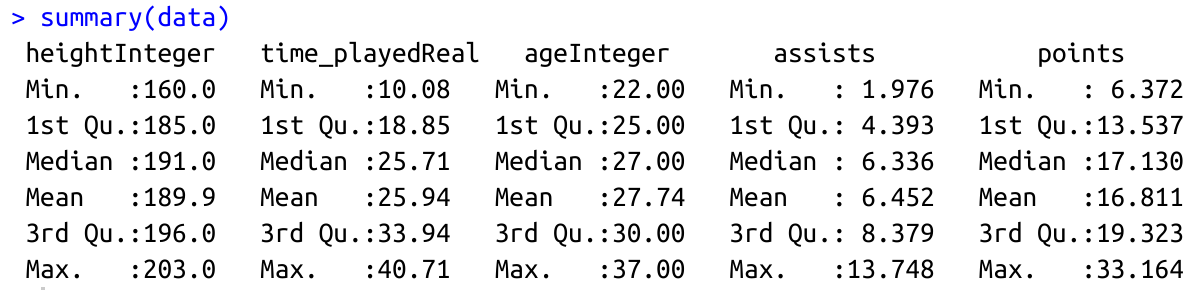
\includegraphics[scale=0.3]{summary.png}  %el parámetro scale permite agrandar o achicar la imagen. En el nombre de archivo puede especificar directorios
	\caption{Resumen estadístico de las variables} 
	\label{fig:summary}
\end{figure}

\subsection{Esquema de trabajo}

Presento tres aproximaciones en la búsqueda de reglas de asociación interesantes. La primera de ellas se basa en la forma clásica: defino una partición de datos, genero transacciones y aplico el algoritmo Apriori para encontrar itemsets frecuentes y reglas de asociación. Ante la problemática de definir una partición correcta, en la segunda aproximación aplico MOPNAR para encontrar la partición óptima según el algoritmo. Por último, contemplo el caso en que la división del conjunto de datos no sea una partición sino un recubrimiento, es decir, la intersección de los intervalos no es vacía. Así, puedo generar reglas afirmativas y negativas (como en el caso de MOPNAR) y estudiar conjuntos de reglas con las pautas dadas en el curso. 

\section{Primera aproximación: Partición de datos y búsqueda de reglas con Apriori}



\section{Segunda aproximación: MOPNAR y búsqueda de reglas}



\section{Tercera aproximación: Recubrimiento de datos, items negados y conjuntos de reglas}


\newpage
\section{Bibliografía}

%------------------------------------------------

\bibliography{citas} %archivo citas.bib que contiene las entradas 
\bibliographystyle{plain} % hay varias formas de citar

\end{document}
